\documentclass[a4paper,11pt]{article}
\usepackage{amsmath,amsthm,amsfonts,amssymb,amscd,amstext,vmargin,graphics,graphicx,tabularx,multicol} 
\usepackage[francais]{babel}
\usepackage[utf8]{inputenc}  
\usepackage[T1]{fontenc} 
\usepackage{pstricks-add,tikz,tkz-tab,variations}
\usepackage[autolanguage,np]{numprint} 
\usepackage{calc}

\setmarginsrb{1.5cm}{0.5cm}{1cm}{0.5cm}{0cm}{0cm}{0cm}{0cm} %Gauche, haut, droite, haut
\newcounter{numexo}
\newcommand{\exo}[1]{\stepcounter{numexo}\noindent{\bf Exercice~\thenumexo} : }
\reversemarginpar

\newcommand{\bmul}[1]{\begin{multicols}{#1}}
\newcommand{\emul}{\end{multicols}}

\newcounter{enumtabi}
\newcounter{enumtaba}
\newcommand{\q}{\stepcounter{enumtabi} \theenumtabi.  }
\newcommand{\qa}{\stepcounter{enumtaba} (\alph{enumtaba}) }
\newcommand{\initq}{\setcounter{enumtabi}{0}}
\newcommand{\initqa}{\setcounter{enumtaba}{0}}

\newcommand{\be}{\begin{enumerate}}
\newcommand{\ee}{\end{enumerate}}
\newcommand{\bi}{\begin{itemize}}
\newcommand{\ei}{\end{itemize}}
\newcommand{\bp}{\begin{pspicture*}}
\newcommand{\ep}{\end{pspicture*}}
\newcommand{\bt}{\begin{tabular}}
\newcommand{\et}{\end{tabular}}
\renewcommand{\tabularxcolumn}[1]{>{\centering}m{#1}} %(colonne m{} centrée, au lieu de p par défault) 
\newcommand{\tnl}{\tabularnewline}

\newcommand{\trait}{\noindent \rule{\linewidth}{0.2mm}}
\newcommand{\hs}[1]{\hspace{#1}}
\newcommand{\vs}[1]{\vspace{#1}}

\newcommand{\N}{\mathbb{N}}
\newcommand{\Z}{\mathbb{Z}}
\newcommand{\R}{\mathbb{R}}
\newcommand{\C}{\mathbb{C}}
\newcommand{\Dcal}{\mathcal{D}}
\newcommand{\Ccal}{\mathcal{C}}
\newcommand{\mc}{\mathcal}

\newcommand{\vect}[1]{\overrightarrow{#1}}
\newcommand{\ds}{\displaystyle}
\newcommand{\eq}{\quad \Leftrightarrow \quad}
\newcommand{\vecti}{\vec{\imath}}
\newcommand{\vectj}{\vec{\jmath}}
\newcommand{\Oij}{(O;\vec{\imath}, \vec{\jmath})}
\newcommand{\OIJ}{(O;I,J)}


\newcommand{\reponse}[1][1]{%
\multido{}{#1}{\makebox[\linewidth]{\rule[0pt]{0pt}{20pt}\dotfill}
}}

\newcommand{\titre}[5] 
% #1: titre #2: haut gauche #3: bas gauche #4: haut droite #5: bas droite
{
\noindent #2 \hfill #4 \\
#3 \hfill #5

\vspace{-1.6cm}

\begin{center}\rule{6cm}{0.5mm}\end{center}
\vspace{0.2cm}
\begin{center}{\large{\textbf{#1}}}\end{center}
\begin{center}\rule{6cm}{0.5mm}\end{center}
}



\begin{document}
\pagestyle{empty}
\titre{Séance d'AP  . . . : Le théorème de Thalès}{}{}{3ème}{}

\vspace*{0.2cm}

\setlength{\fboxrule}{2pt}
\begin{flushleft}
\framebox{\begin{minipage}{\linewidth}



\begin{center}
\underline{\textbf{{\large Rappels de cours}}}
\end{center}


\textbf{\underline{Exemple de résolution :}}
\bmul{2}

\includegraphics[scale=0.4]{thalesap2.eps} \\
Dans la figure ci-dessous, les droites (MN) et (BC) sont parallèles.\\
\textbf{Calculer la longueur AC.}

\columnbreak

Dans le triangle ABC :
\bi
\item Les droites (AB) et (AC) sont sécantes en A.
\item (MN) $\slash\slash$ (BC)\\
\ei

D'après le théorème de Thalès, on a:

\begin{center}
$\dfrac{AM}{AB}=\dfrac{AN}{AC}=\dfrac{MN}{BC}$\\
\end{center}
 



On remplace : \hspace*{1cm} $\dfrac{10}{16}=\dfrac{8}{AC}=\dfrac{MN}{7,2}$\\


\textbf{Calcul de AC :}\\

$\dfrac{10}{16}=\dfrac{8}{AC}$ donc $AC = \dfrac{8 \times 16}{10}$\\

\fbox{AC = 12,8 cm} 


\emul




\vspace*{0.2cm}
\end{minipage}}
\end{flushleft}

\vspace*{0.4cm}
\exo \\
On suppose que les droites (BE) et (PM) sont parallèles ainsi que les droites (LB) et (IC).\\
Écrire les égalités données par le théorème de Thalès dans les cas suivants :

\includegraphics[scale=0.6]{papillon1.eps} \hspace*{6cm} \includegraphics[scale=0.6]{thales5.eps} 

\bmul{2}

\exo \\

\includegraphics[scale=0.4]{thalesap1.eps} 

Dans la figure ci-contre, les droites (DE) et (BC) sont parallèles.\\
\textbf{Calculer les longueurs DE et AE.}\\




\columnbreak

\exo \\

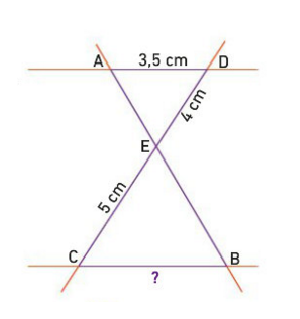
\includegraphics[scale=1.1]{papillon.eps} 



On considère le triangle ci-contre, les droites (AD) et (BC) sont parallèles. \\
\textbf{Calculer la distance BC.}


 \emul
 
\newpage 
 
\textbf{\underline{Exercice :}}
 
 \includegraphics[scale=0.6]{thalesap.eps} \\
 
 \vspace*{0.75cm}
 
 
\textbf{\underline{Exercice :}}

 \includegraphics[scale=0.6]{thalesap.eps} \\

 \vspace*{0.75cm}
 
\textbf{\underline{Exercice :}}
 
 \includegraphics[scale=0.6]{thalesap.eps} 
 

\end{document}
